\section*{Introduction du chapitre}

	L'objet de ce chapitre est de présenter la démarche méthodologique suivie. La thèse se structure autour de deux études. Dans les parties précédentes, nous avons souligné l'intérêt d'envisager l'action environnementale à la fois à travers le spectre du discours et de la communication, et celui de la pratique. Les études menées traitent de ces deux aspects, en mobilisant à la fois de méthodes quantitatives et qualitatives. Les approches de ce types sont qualifiées de \cit{Méthodes mixtes} \parencite{aldebert2011utilisation}. De plus en plus utilisées dans les articles en sciences de gestion, elles répondent à plusieurs besoins \parencite{pascal2018les}. Les auteures recensent des bénéfices en termes de complémentarité, de complétude, de corroboration, d'expansion (c'est à dire l'enrichissement des résultats par une autre méthode) et de développement. Elles soulignent en outre que les méthodes mixtes sont fréquemment utilisées dans une approche positiviste ou post-positiviste, bien que les auteurs s'appuient également sur d'autres paradigmes épistémologiques, voire sur une démarche purement pragmatique. \textcite{klassen2012best, creswell2010designing} proposent plusieurs designs méthodologiques correspondant aux différents besoins de la recherche. Celui adopté ici est un design \cit{convergent} qui vise à s'appuyer sur des données différentes pour aboutir à une meilleure compréhension du sujet \parencite{pascal2018les}. Ce design est adapté à une situation dans laquelle la littérature est encore peu développée. En effet, si l’action environnementale fait l’objet de nombreux travaux académiques, ceux-ci portent généralement sur le secteur lucratif et sont difficilement transposables aux nombreuses particularités de l’ESS. Il est donc utile de l'aborder sous différents angles pour en obtenir une meilleure compréhension. Conformément à ce type de démarche, les deux études sont menées de manière simultanée et indépendante. Les résultats sont discutés séparément avant de donner lieu à une analyse générale bénéficiant des apports des deux études (phase d'intégration, chapitre \ref{chapitre:discussion}).	\\

\begin{landscape}
    \begin{figure}
        \centering
        \caption{Démarche méthodologique}
        \label{fig:methodoglobale}
        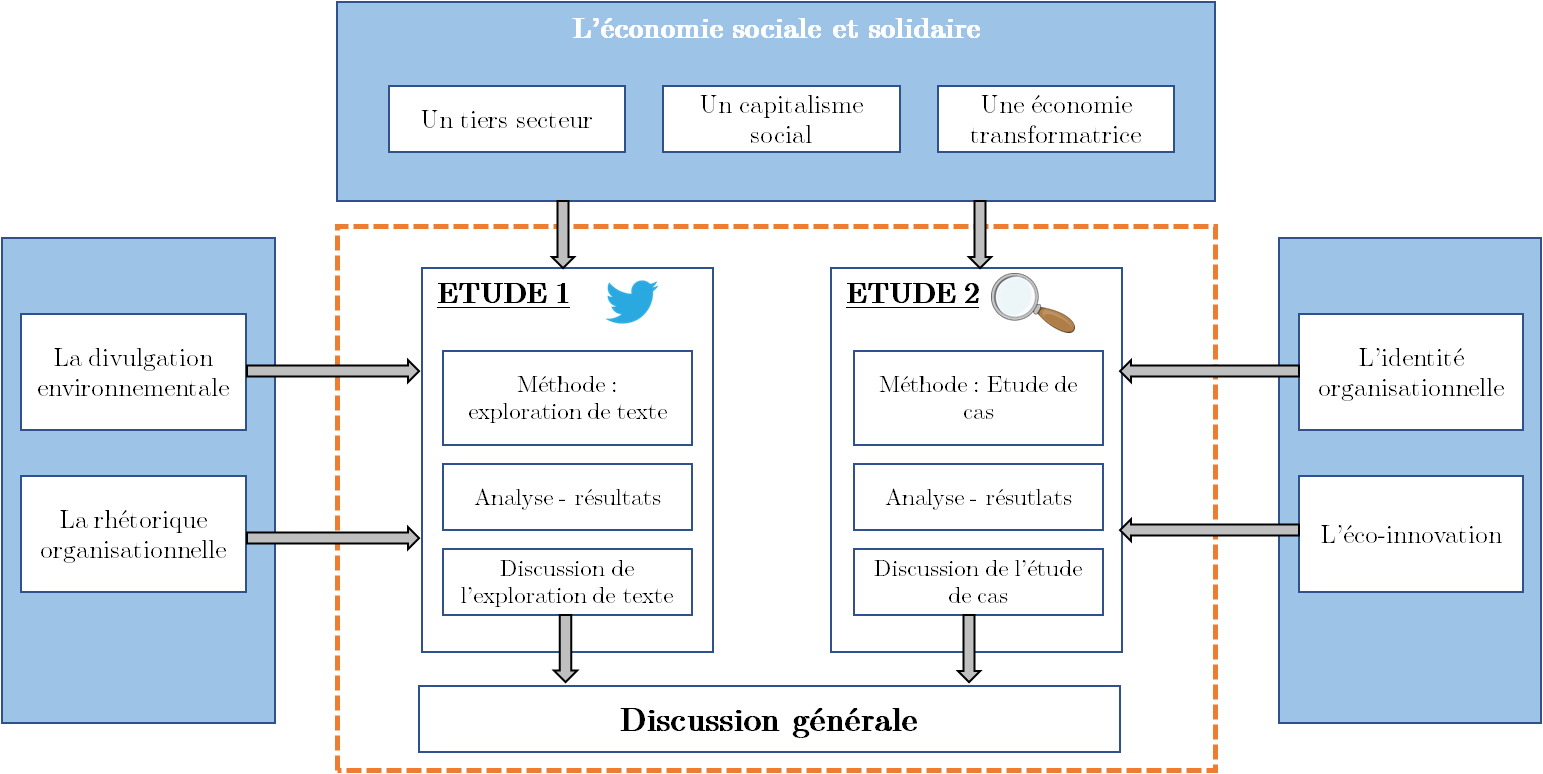
\includegraphics[width=\linewidth]{fig/methodo.png}
    \end{figure}
\end{landscape}

	La figure \ref{fig:methodoglobale} présente l'agencement général de la recherche. La première étude (chapitre \ref{chapitre:twitter}) porte sur la communication environnementale des \eess sur un réseau social destiné à tous les publics : Twitter. Nous mobilisons les méthodes de l’exploration de texte pour traiter un corpus de plus de 28 000 messages relatifs à l’environnement postés sur ce réseau. La seconde étude porte sur plusieurs cas, dans le but d'identifier, au-delà du discours, la façon dont les \eess peuvent effectivement agir pour protéger l’environnement. L’étude des cas se base sur les documents de référence des entreprises, leur site internet ainsi que sur une série d’entretiens auprès de dirigeants. \\
